\documentclass[a4paper,12pt]{article}

% Packages
\usepackage[utf8]{inputenc}
\usepackage{geometry}
\usepackage{titlesec}
\usepackage{lipsum} % for generating dummy text
\usepackage{graphicx}
\usepackage{caption}
\usepackage{subcaption}
\usepackage{listings}
\usepackage{amsmath}
\usepackage{amssymb}                                                                                                                                                            
\usepackage{xcolor}

% Page setup
\geometry{a4paper, margin=1in}
\setlength{\parindent}{0pt}
\setlength{\parskip}{5pt}

% Title setup
\title{\textbf{DSP LAB - Experiment 6} \\
        \vspace*{0.3em}
        \large{Discrete Time Fourier Transform (DTFT)} \\}                                              
\author{Ajay Krishnan K \\  EE22BTECH11003}
\date{\today}

% Section and subsection formatting
\titleformat{\section}[block]{\normalfont\Large\bfseries}{\thesection}{1em}{}
\titleformat{\subsection}[block]{\normalfont\large\bfseries}{\thesubsection}{1em}{}
\titleformat{\subsubsection}[block]{\normalfont\normalsize\bfseries}{\thesubsubsection}{1em}{}

% Code listing settings
\lstdefinestyle{mystyle}{
    language=Matlab,
    basicstyle=\ttfamily\small,
    breaklines=true,
    keywordstyle=\color{blue},
    commentstyle=\color{green!40!black},
    stringstyle=\color{red},
    % numbers=left,
    % numberstyle=\tiny,
    frame=single,
    showspaces=false,
    showstringspaces=false,
}

\lstset{style=mystyle}

\begin{document}
\maketitle

\section*{Aim}
To compute the Discrete Time Fourier Transform (DTFT) of a given sequence.

\section*{Theory}
The Discrete Time Fourier Transform (DTFT) of a sequence $x[n]$ is given by
\begin{equation}
    % X(w) = \sum_{n=-\infty}^{\infty} x[n] e^{-j\omega n}
    X(\omega) = \sum_{n=-\infty}^{\infty} x[n] e^{-j\omega n}
\end{equation}
% where $X(w)$ is a continuous function of $\omega$.
where $X(\omega)$ is a continuous function of $\omega$.

The DTFT of a sequence is a continuous function of frequency and is periodic with period $2\pi$.
It provides the frequency content of the given sequence $x[n]$. The magnitude of $X(w)$ gives the strength of the frequency components and the phase of $X(w)$ gives the phase shift of the frequency components.


\section*{Procedure}
The DTFT of a given sequence can be computed using the following steps:
\begin{enumerate}
    \item Generate the sequence $x[n]$.
    \item Compute the DTFT $X(w)$ using the formula (1).
    \item Plot the $X(w)$.
\end{enumerate}

\section*{Implementation}
The following MATLAB code computes the DTFT of a given sequence $x[n]$ and plots $X(w)$.

\lstinputlisting[language=Matlab]{../code/dtft_test.m}

\section*{Results}
The DTFT of the given sequence $x[n]$ is computed and plotted. The magnitude plot of $X(w)$ is shown in the figure below.

\begin{figure}[ht]
    \centering
    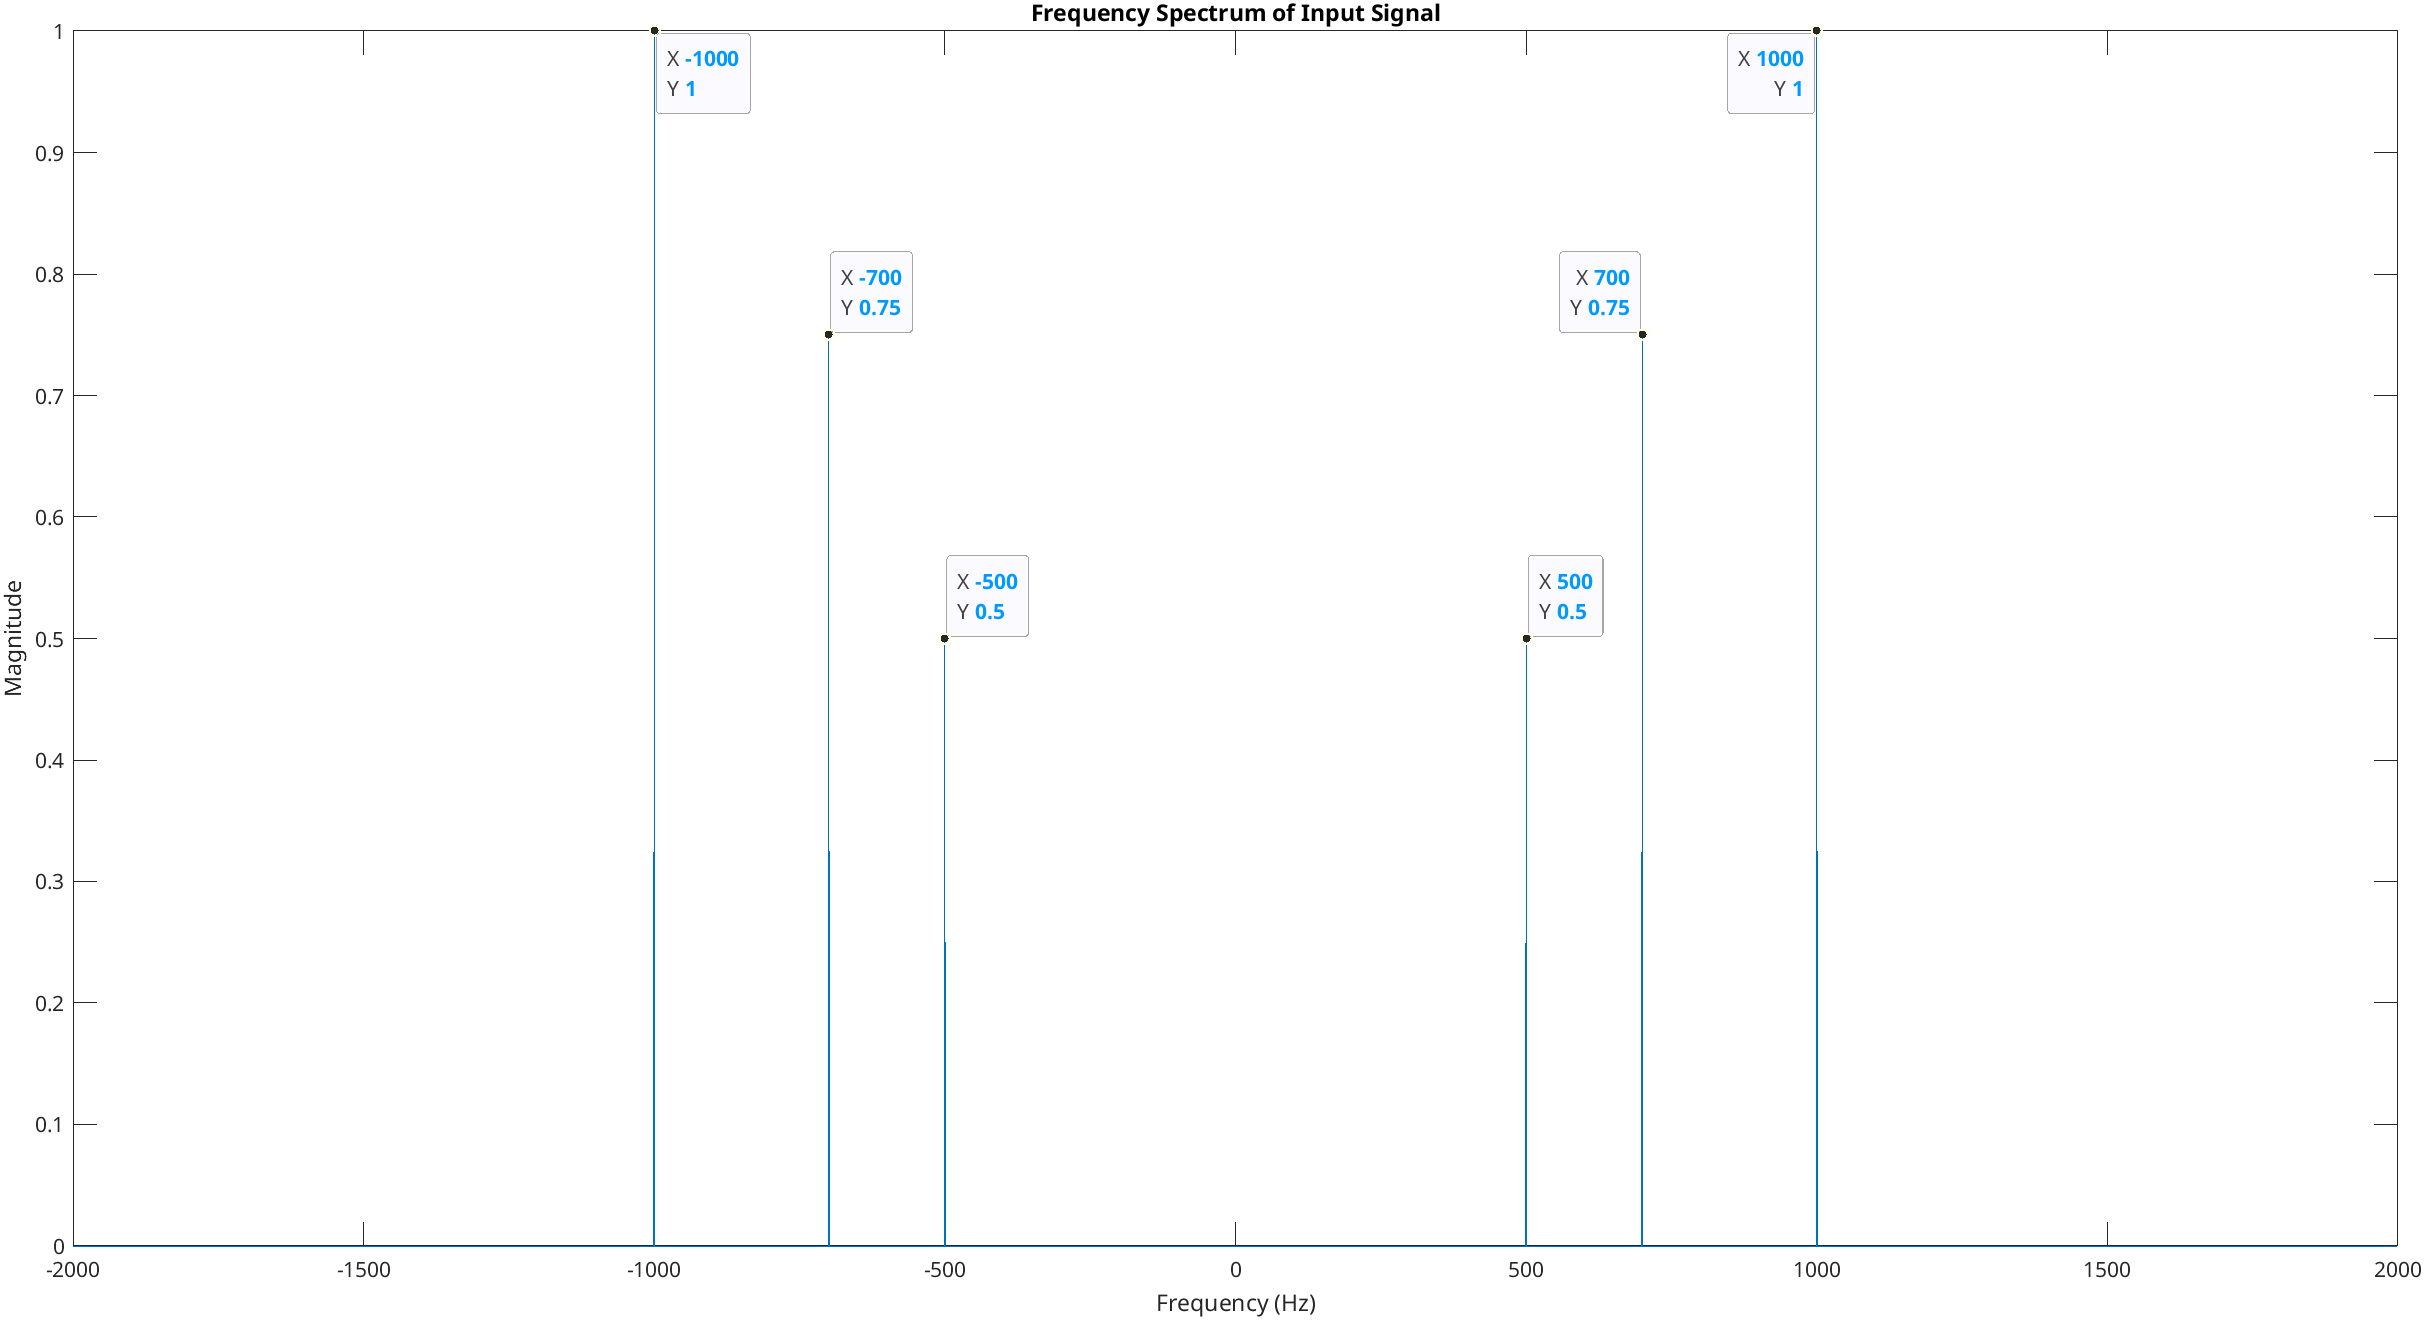
\includegraphics[width=0.8\textwidth]{./figs/dtft.png}
    \caption{Magnitude of $X(w)$}
    \label{fig:dtft}
\end{figure}

\section*{Observations}
The magnitude of $X(w)$ is plotted in Fig. \ref{fig:dtft}.
 The figure shows three peaks at $f = 500 Hz$, $f = 1000 Hz$ and $f = 700 Hz$ (same at the negative frequencies),
 with magnitudes $|X(w)| = 0.5$, $|X(w)| = 1$ and $|X(w)| = 0.75$ respectively. This indicates the presence of frequency components at these frequencies in the input sequence $x[n]$.
 This magnitudes are also consistent with the input sequence $x[n]$.

\section*{Conclusion}
The Discrete Time Fourier Transform (DTFT) of a given sequence has been computed and plotted.
 This method can be used to analyze the frequency content of a given sequence.
 From the plot, we can observe the frequency components present in the input sequence and the 
 magnitude of $X(w)$ is consistent with the input sequence $x[n]$.
\end{document}